\section{Exemplos de Aplicações}
\label{s.applications}

\begin{frame}{Exemplos de Aplicações}
	\justifying
	A otimização meta-heurística possui uma vasta gama de aplicações, tais como:
	\\~\\
	\begin{itemize}
		\justifying
		\item Otimização de funções matemáticas;
		\\~\\
		\item Otimização de hiperparâmetros;
		\\~\\
		\item Seleção de características;
		\\~\\
		\item \sout{Seleção de modelos}.
	\end{itemize}
\end{frame}

\begin{frame}
	\justifying
	A implementação deste mini-curso está disponível no GitHub\footnote{\url{https://github.com/gugarosa/mh_deep_application}} e utiliza as seguintes bibliotecas:
	\\~\\
	\begin{itemize}
		\justifying
		\item Opytimizer\footnote{\url{https://github.com/gugarosa/opytimizer}};
		\\~\\
		\item Scikit-learn\footnote{\url{https://scikit-learn.org}};
		\\~\\
		\item PyTorch\footnote{\url{https://pytorch.org}}.
	\end{itemize}
\end{frame}


\subsection{Otimização de Funções Matemáticas}
\label{ss.applications_benchmark}

\begin{frame}{Otimização de Funções Matemáticas}
	\begin{figure}
		\centering
		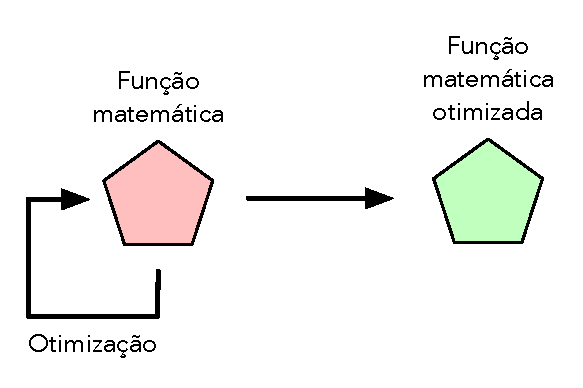
\includegraphics[scale=0.6]{figs/benchmark_opt.eps}	
		\caption{Fluxograma do processo de otimização de funções matemáticas.}
		\label{f.benchmark_opt}
	\end{figure}
	Códigos: \url{https://github.com/gugarosa/mh_deep_application/tree/main/applications/meta_heuristic}
\end{frame}

\subsection{Otimização de Hiperparâmetros}
\label{ss.applications_hyperparameter}

\begin{frame}{Otimização de Hiperparâmetros}
	\begin{figure}
		\centering
		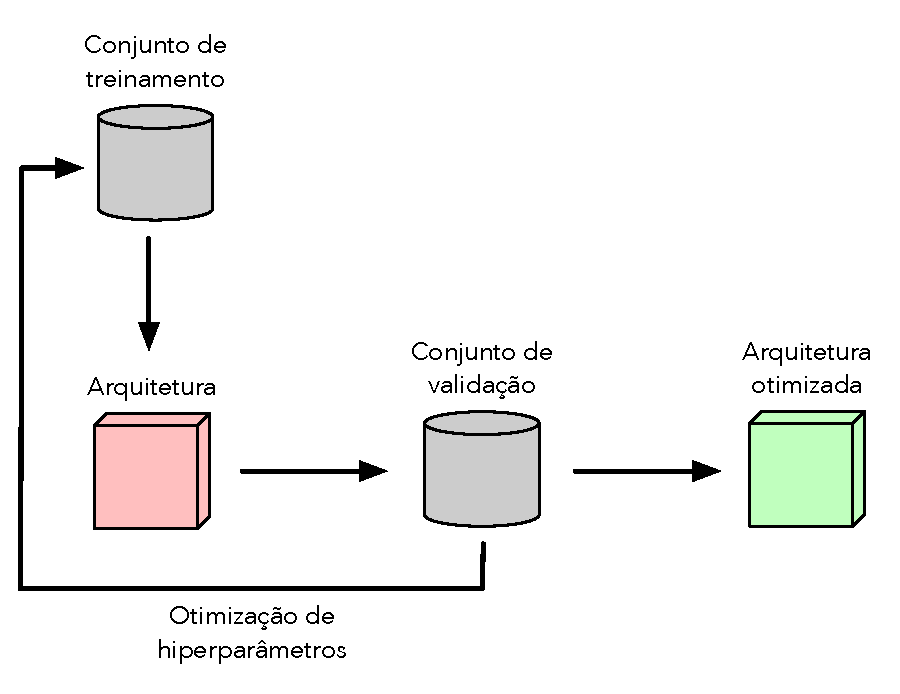
\includegraphics[scale=0.45]{figs/hyperparameter_opt.eps}	
		\caption{Fluxograma do processo de otimização de hiperparâmetros.}
		\label{f.hyperparameter_opt}
	\end{figure}
	Códigos: \url{https://github.com/gugarosa/mh_deep_application/tree/main/applications/hyperparameter_optimization}
\end{frame}

\subsection{Seleção de Características}
\label{ss.applications_feature_selection}

\begin{frame}{Seleção de Características}
	\begin{figure}
		\centering
		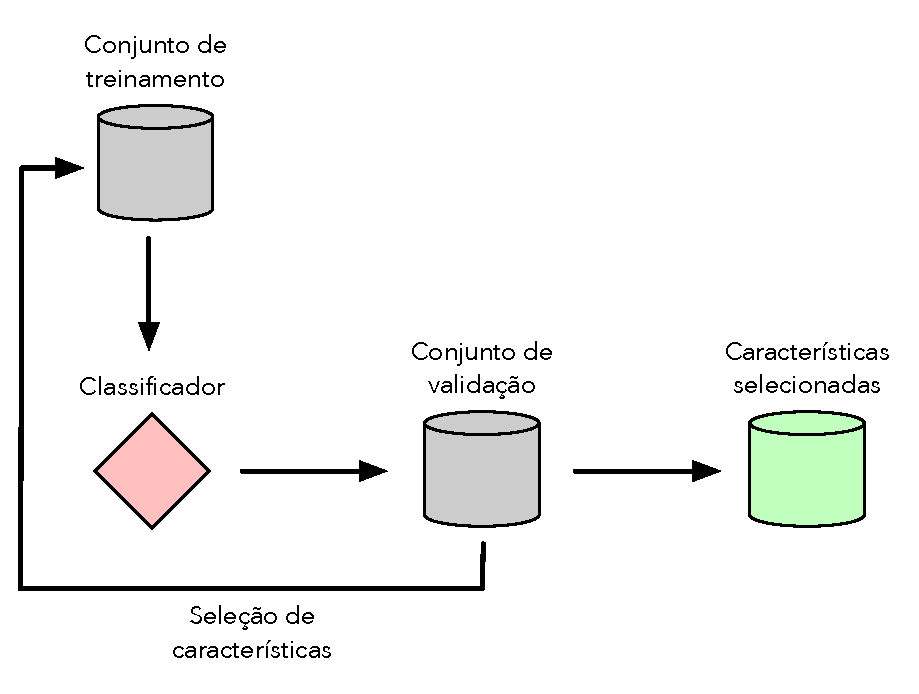
\includegraphics[scale=0.45]{figs/feature_selection.eps}	
		\caption{Fluxograma do processo de seleção de características.}
		\label{f.feature_selection}
	\end{figure}
	Códigos: \url{https://github.com/gugarosa/mh_deep_application/tree/main/applications/feature_selection}
\end{frame}